\chapter{Additional experiments}

\section{Experiment with static point}

\subsection*{16~cm setup}
\label{ss:16results}
Here we provide additional results for the experiment mentioned in the Section
\ref{s:experiment-static}. The box plots for distances from the left column
(\ref{fig:verticalleft-boxplot}), from the right column
(\ref{fig:verticalright-boxplot}) and for the perpendicular plane
(\ref{fig:table-boxplot}) are available.

\begin{figure}
\includegraphics[width=\linewidth]{experiments/leftcolumn1.eps}
\caption{Boxplot of relative errors of estimated vertical distances in the left column (experiment with parallel setup)}
\label{fig:verticalleft-boxplot}
\end{figure}

\begin{figure}
\includegraphics[width=\linewidth]{experiments/rightcolumn1.eps}
\caption{Boxplot of relative errors of estimated vertical distances in the right column (experiment with parallel setup)}
\label{fig:verticalright-boxplot}
\end{figure}

\begin{figure}
\includegraphics[width=\linewidth]{experiments/table1.eps}
\caption{Boxplot of relative errors of estimated distances for perpendicular plane (experiment with parallel setup)}
\label{fig:table-boxplot}
\end{figure}


\subsection*{63~cm setup}
\label{ss:63results}

Same experiment described in the Section \ref{s:experiment-static} we tried
with another camera setup. This time the cameras were approximately 63~cm apart
from each other and their views were non-parallel. Same numbering of the grid
points is used in this setup as in the parallel setup.
\newline
Results include:
\begin{itemize}
\item table summarizing an average error and its standart deviation for all distances (\ref{table:63}),
\item box plot for distances of the horizontal lines (\ref{table:63horizontal}),
\item box plot for distances of the vertical lines in the left column (\ref{table:63left}),
\item box plot for distances of the vertical lines in the right column (\ref{table:63right}),
\item box plot for distances of the lines in perpendicular plane (\ref{table:63table}).
\end{itemize}

\begin{table}
\centering
\begin{tabular}{|r|r|r|r|r|r|}
\hline
\multicolumn{2}{|c|}{Points} & \multicolumn{1}{c|}{Real} & \multicolumn{3}{c|}{Error} \\
\cline{1-2} \cline{4-6}
From & To & length [mm] & Average [mm] & Average [\%] & Std. dev. [mm]\\
\hline
\hline
\input{experiments/63/distances.txt}
\hline
\end{tabular}
\caption{Results of the experiment focused on the distances}
\label{table:63}
\end{table}

\begin{figure}
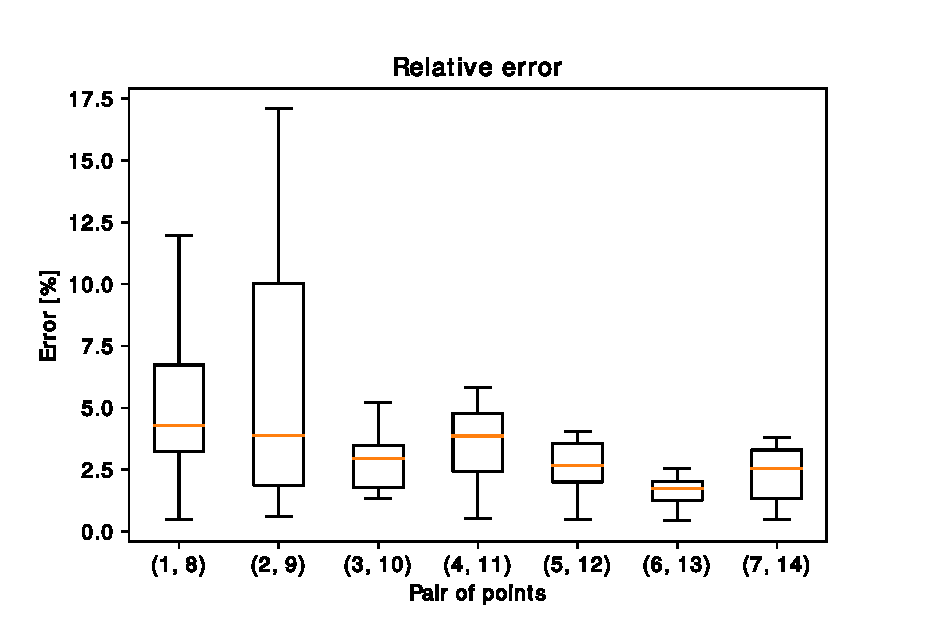
\includegraphics[width=\linewidth]{experiments/63/horizontal1.eps}
\caption{Box plot of relative errors of estimated horizontal distances between the columns (non-parallel setup)}
\label{table:63horizontal}
\end{figure}

\begin{figure}
\includegraphics[width=\linewidth]{experiments/63/leftcolumn1.eps}
\caption{Boxplot of relative errors of estimated vertical distances in the left column (non-parallel setup)}
\label{table:63left}
\end{figure}

\begin{figure}
\includegraphics[width=\linewidth]{experiments/63/rightcolumn1.eps}
\caption{Boxplot of relative errors of estimated vertical distances in the right column (non-parallel setup)}
\label{table:63right}
\end{figure}

\begin{figure}
\includegraphics[width=\linewidth]{experiments/63/table1.eps}
\caption{Boxplot of relative errors of estimated distances in the perpendicular plane (non-parallel setup)}
\label{table:63table}
\end{figure}

\section{Experiment with partial occlusion}

In the experiment we tested trackers under partial occlusion. The results are
displayed in the Table \ref{table:partial-occlusion} and the setup is shown in
the Figure \ref{fig:partial-occlusion}. We remind that the $X$ means the
inacuraccy between the representative tracker and tested tracker. We compute
its sample mean and sample standart deviation. In this experiment the \hsv{}
tracker performed best so we choose it as representative tracker. The
\simback{} background had many problems wiht changing light.

\begin{table}
\centering
\begin{tabular}{l|r|r|r|p{4cm}}
Tracker & Speed [FPS] & $\bar{X}$ [px] & $\sigma_X$ [px] &  Recovers from occlusion (ratio of successful tracking) \\
\hline
\boost{} & 19.65 & 208.14 & 153.63 & No (18.60\%) \\
\corr{} & 110.34 & 168.71 & 94.59 & No (23.75\%)\\
\hsv{} & 507.25 & 0.00 & 0.00 & Yes (100.00\%) \\
\medflow{} & 339.23 & 139.48 & 102.12 & No (40.34\%) \\
\mil{} & 12.67 & 164.94 & 89.61 &  No (21.75\%)\\
\mosse{} & 522.00 & 157.59 & 144.83 & No (32.55\%) \\
\patt{} & 151.22 & 47.72 & 20.77 & Yes (91.56\%)\\
\simback{} & 120.96 & 42.15 & 12.29 & Yes (100\%)\\
\tld{} & 16.72 & 43.46 & 18.08 & Yes (96.92\%)\\
\end{tabular}
\caption{Comparison of trackers under partial occlusion}
\label{table:partial-occlusion}
\end{table}


\section{Experiment under full occlusion}

Similarly to the experiment mentioned in the Chapter \ref{ch:tracker} we did
another experiment with full occlusion. This time, the direction of the robot
is preserved. The results are listed in the Table \ref{fig:full-occlusion} and
the setup is displayed in the image \ref{fig:full-occlusion}. The \hsv{}
tracker is choosed as representative tracker.

\begin{table}
\centering
\begin{tabular}{l|p{1.2cm}|r|r|p{2.5cm}|p{3.5cm}}
Tracker & Speed [FPS] & $\bar{X}$ [px] & $\sigma_X$ [px]&  Report occlusion (ratio of reported) & Recovers from full occlusion (ratio of successful tracking) \\
\hline
\boost{} & 15.61 & 137.07 & 91.90 & No (0\%) & No (17.46\%) \\
\corr{} & 108.89 & 123.82 & 75.17 & No (0\%) & No (16.42\%) \\
\hsv{} & 498.31 & 0.00 & 0.00 & Yes (100\%) & Yes (100\%) \\
\medflow{} & 318.07 & 121.08 & 74.70 & No (2.90\%) & No (16.22\%) \\
\mil{} & 10.50 & 122.69 & 87.34 & No (0\%) & No (16.84\%) \\
\mosse{} & 789.96 & 106.57 & 89.99 & No (0\%) & No (33.78\%) \\
Pattern m. & 149.14 & 26.53 & 7.81 & No (0\%) & Yes (100\%) \\
Simple b. & 118.94 & 84.59 & 67.21 & No (0\%) & No (41.68\%) \\
\tld{} & 15.66 & 30.39 & 10.94 & No (0\%) & Yes (100\%) \\
\end{tabular}
\caption{Comparison of trackers under full occlusion}
\label{table:full-occlusion}
\end{table}

\begin{figure}
\centering
\begin{subfigure}{0.48\linewidth}
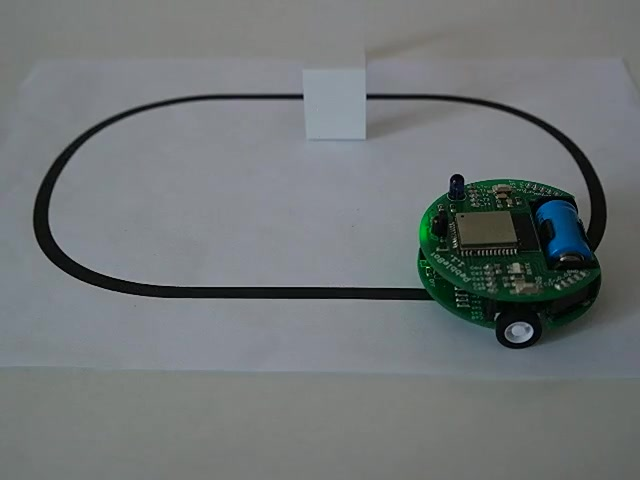
\includegraphics[width=\linewidth]{img/experiments/partial-occlusion.jpg}
\caption{Setup for partial occlusion}
\label{fig:partial-occlusion}
\end{subfigure}
\begin{subfigure}{0.48\linewidth}
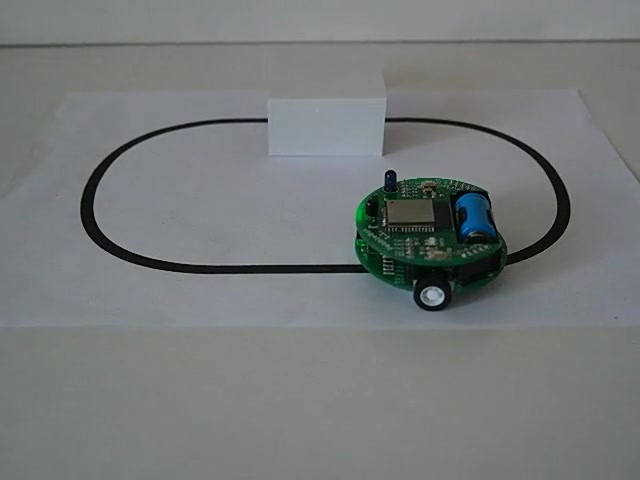
\includegraphics[width=\linewidth]{img/experiments/full-occlusion.jpg}
\caption{Setup for full occlusion}
\label{fig:full-occlusion}
\end{subfigure}
\caption{Setups used for testing trackers performance under occlusion}
\label{fig:additional-occlusion}
\end{figure}
